% CARICA IL LAYOUT PER IL DOCUMENTO
\documentclass[11pt,a4paper]{article}
\usepackage[a4paper,portrait,top=3.5cm,bottom=3.5cm,left=3cm,right=3cm,bindingoffset=5mm]{geometry}
\usepackage[T1]{fontenc}
\usepackage[utf8x]{inputenc}
\usepackage{graphicx}
\usepackage{caption}
\usepackage[italian]{babel}
\usepackage{listings}
\usepackage{fancyhdr}
\usepackage{lastpage}
\usepackage{hyperref}
\usepackage{array,booktabs}
\usepackage{subcaption}

% Identazione tabella gruppo Frontespizio.tex
\newcolumntype{L}[1]{>{\raggedright\let\newline\\\arraybackslash\hspace{0pt}}m{#1}}
\newcolumntype{C}[1]{>{\centering\let\newline\\\arraybackslash\hspace{0pt}}m{#1}}
\newcolumntype{R}[1]{>{\raggedleft\let\newline\\\arraybackslash\hspace{0pt}}m{#1}}

% Header and Footer

\fancypagestyle{std}{
	\fancyhf{}
	\lhead{
\includegraphics[width=1.7cm]{images/frontImage.png}}
	\chead{}
	\rhead {\nouppercase{\leftmark}}
	\lfoot{}
	\cfoot{}
	\rfoot{Pagina \thepage\ di \pageref{LastPage}}
	\renewcommand{\headrulewidth}{0.3pt}
	\renewcommand{\footrulewidth}{0.3pt}
}

\fancypagestyle{romano}{
	\fancyhf{}
	\lhead{
\includegraphics[width=1.7cm]{images/frontImage.png}}
	\chead{}
	\lfoot{}
	\cfoot{}
	\rfoot{}
	\rfoot{\thepage}
	\renewcommand{\headrulewidth}{0.3pt}
	\renewcommand{\footrulewidth}{0.3pt}
}
	
% DEFINIZIONE ELEMENTI FRONTESPIZIO
\title{\bfseries Scherma Castelfranco Veneto}
\author{Chiara Bigarella mat. \\Pavanello Mirko mat. 1009424 \\Massimiliano Sartoretto mat. 1008168,\\ Paolo Tesser mat. 1026527}
\date{A.A. 2013/2014}
\begin{document}
%\maketitle
%\vspace {20 mm}
%
\includegraphics[width=150mm, height=120mm]{images/page_logo.png}
\begin{titlepage}
 \begin{center}
     
\includegraphics[width=8cm]{images/page_logo.png}\\
     
     \vspace{3em} \hrule \vspace{2em}
     {\LARGE \LARGE \LARGE \textbf{Scherma Castelfranco Veneto}}\\
     \vspace{2em} \hrule \vspace{2em}
     \vspace{2em}
 \end{center}

\begin{center}
	{\LARGE { \scshape gruppo L'intrusa}}\\
	\vspace{2em}
    \begin{tabular}{ R{5cm} | L{5cm}  }
    \textbf{Chiara Bigarella} & mat \\ \\
    \textbf{Mirko Pavanello} & mat. 1009424 \\ \\
    \textbf{Massimiliano Sartoretto} & mat. 1008168 \\ \\
    \textbf{Paolo Tesser} &  mat. 1026527 \\ \\
    \end{tabular}
\end{center}

\vskip 0.7cm
\begin{center}
Sommario: \\Relazione del progetto di Tecnologie Web AA 2013-14\\
\end{center}
\end{titlepage}
\newpage


% INDICI DI CONTENUTO E IMMAGINI
\pagestyle{romano}
\pagenumbering{Roman}
\newpage
	\tableofcontents
\newpage
	\listoffigures
\newpage
\pagenumbering{arabic}
\pagestyle{std}

% CORPO DEL DOCUMENTO
\section{Abstract}
Il progetto consiste nella realizzazione del sito della societ\`a sportiva di scherma di Castelfranco Veneto.

\newpage
\section{Accesso al sito}
	Il sito \`e accessibile all'indirizzo web \href{http://tecnologie-web.studenti.math.unipd.it/tecweb/~ptesser/}{http://tecnologie-web.studenti.math.unipd.it/tecweb/~ptesser/}.

\subsection{Amministrazione}
La parte amministrativa \`e accessibile attraverso il link \textit{Area privata} presente in ogni pagina del sito. \\ I dati di accesso sono:
\begin{itemize}
	\item \textbf{username}: admin
	\item \textbf{password}: admin
\end{itemize}

\newpage
\section{Descrizione generale}
	Il gruppo ha deciso di realizzare un sito di pubblicazione di articoli e documenti, per la societ\`a sportiva di scherma di Castelfranco Veneto. Il sito sar\`a composto da una parte utente, accessibile da chiunque, e una parte amministratore, accessibile solamente dalla persona incaricata di pubblicare articoli e documenti. 
Per un utente del sito sar\`a dunque possibile consultare gli articoli recenti, scaricare documenti in formato PDF, e accedere a informazioni pubbliche della societ\`a, mentre l'amministratore potr\`a accedere all'area privata e gestire le risorse pubblicate, inserendo, modificando o eliminando articoli e/o documenti.\\

\noindent La parte utente \`e composta da 7 pagine:
\begin{itemize}
	\item {\bfseries\textit{Articoli}} che mostra gli articoli recentemente inseriti.
	\item {\bfseries\textit{Documenti}} che rende scaricabili dei documenti di interesse.
	\item {\bfseries\textit{Storia}} che descrive la storia della societ\`a.
	\item {\bfseries\textit{Staff}} che mostra le persone che fanno parte dello staff.
	\item {\bfseries\textit{Corsi}} che mostra l'orario dei corsi.
	\item {\bfseries\textit{Login}} che mostra un form di login per l'accesso all'area privata.
\end{itemize}
La parte amministratore \`e composta da 6 pagine:
\begin{itemize}
	\item {\bfseries\textit{InserisciArticolo.cgi}} che permette di inserire un nuovo articolo.
	\item {\bfseries\textit{ModificaArticolo.cgi}} che permette di scegliere un articolo da modificare.
	\item {\bfseries\textit{EliminaArticolo.cgi}} che permette di selezionare articoli da eliminare.
	\item {\bfseries\textit{InserisciDocumento.cgi}} che permette di inserire un nuovo documento.
	\item {\bfseries\textit{ModificaDocumento.cgi}} che permette di scegliere un documento da modificare.
	\item {\bfseries\textit{EliminaDocumento.cgi}} che permette di selezionare documento da eliminare.
\end{itemize}


	
\newpage
\section{Progettazione}
	\subsection{Struttura}
		\subsubsection{Definizione}
	\noindent La parte \underline{utente} \`e composta da 7 pagine:
\begin{itemize}
	\item {\bfseries\textit{Articoli}} che mostra gli articoli recentemente inseriti.
	\item {\bfseries\textit{Articolo}} che mostra un singolo articolo selezionato.
	\item {\bfseries\textit{Documenti}} che rende scaricabili dei documenti di interesse.
	\item {\bfseries\textit{Storia}} che descrive la storia della societ\`a.
	\item {\bfseries\textit{Staff}} che mostra le persone che fanno parte dello staff.
	\item {\bfseries\textit{Corsi}} che mostra l'orario dei corsi.
	\item {\bfseries\textit{Login}} che mostra un form di login per l'accesso all'area privata.
\end{itemize}
	In particolare le pagine \textit{staff.html}, \textit{storia.html} e \textit{corsi.html} sono statiche, mentre le altre pagine sono state ottenute attraverso l'associazione dei file xml ad un foglio di stile e la stampa tramite Perl.

La parte \underline{amministratore} \`e composta da 6 pagine:
\begin{itemize}
	\item {\bfseries\textit{InserisciArticolo.cgi}} che permette di inserire un nuovo articolo.
	\item {\bfseries\textit{ModificaArticolo.cgi}} che permette di scegliere un articolo da modificare.
	\item {\bfseries\textit{EliminaArticolo.cgi}} che permette di selezionare articoli da eliminare.
	\item {\bfseries\textit{InserisciDocumento.cgi}} che permette di inserire un nuovo documento.
	\item {\bfseries\textit{ModificaDocumento.cgi}} che permette di scegliere un documento da modificare.
	\item {\bfseries\textit{EliminaDocumento.cgi}} che permette di selezionare documento da eliminare.
\end{itemize}	
	
	Tutte queste pagine sono dinamiche, create in Perl come composizione di documenti definiti in XHTML e istruzioni Perl.
	
\subsubsection{Database}
	La persistenza dei data \`e ottenuta attraverso due file XML validi secondo gli schemi definiti in \textit{articoli.xsl} e \textit{documenti.xsd}. Si \`e scelto XML Schema poich\`e garantisce l'espressivit\`a di cui abbiamo bisogno, in particolare per avere a disposizione i primitivi date e anyURI, utili nella definizione di articoli e documenti.
	\subsection{Presentazione}
		Abbiamo previsto tre layout differenti basati sulla dimensione dello schermo del device.
%\begin{figure}[h]
%        \centering
%        \begin{subfigure}[b]{0.10\textwidth}
%		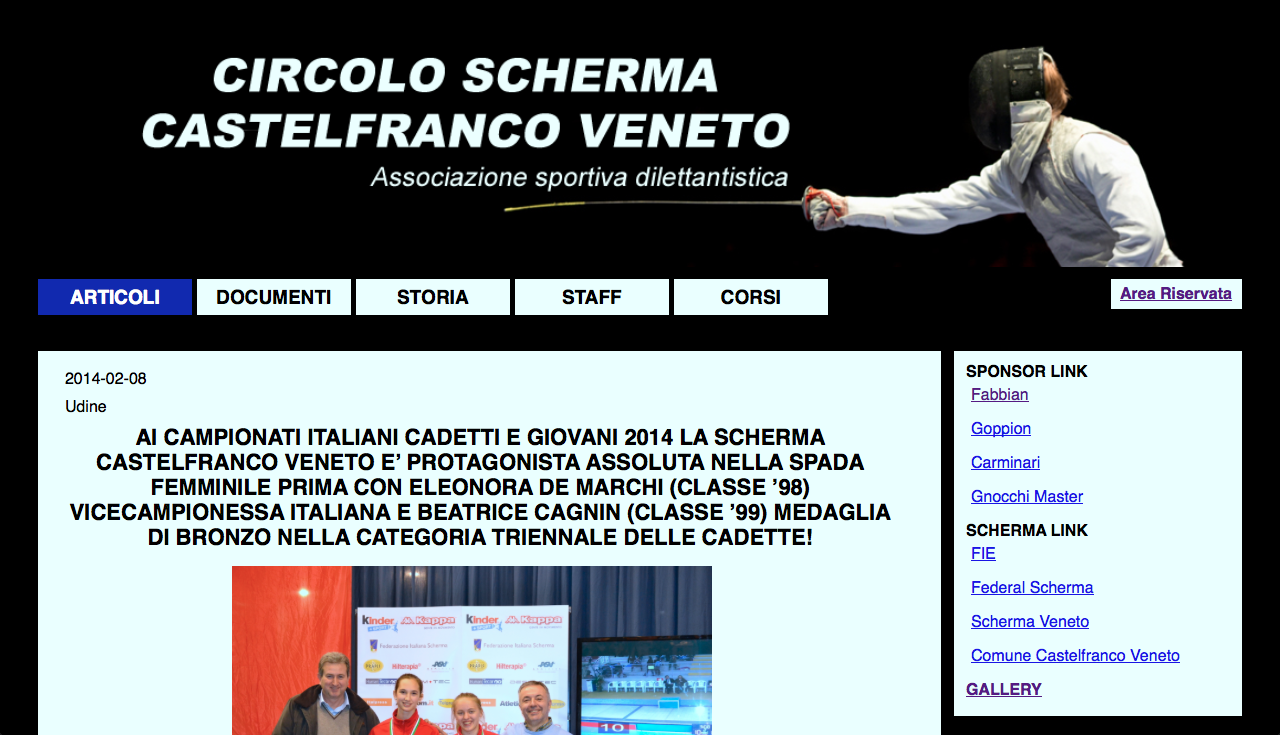
\includegraphics[scale=0.32]{images/articoli_desktop.png}
%		\caption{Screenshot desktop articoli.cgi}
%        \end{subfigure}
%        ~
%        \begin{subfigure}[b]{0.10\textwidth}
%		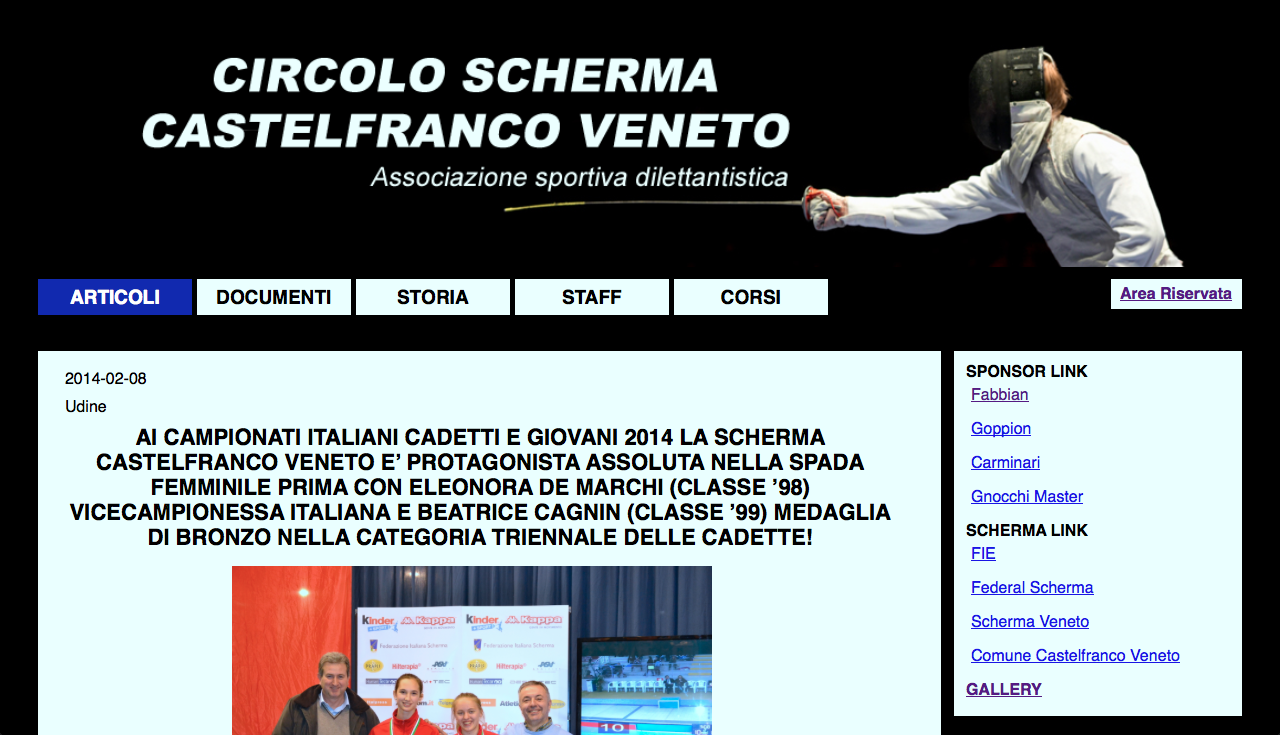
\includegraphics[scale=0.30]{images/articoli_tablet.png}
%		\caption{Screenshot tablet articoli.cgi}
%        \end{subfigure}
%        ~
%        \begin{subfigure}[b]{0.30\textwidth}
%		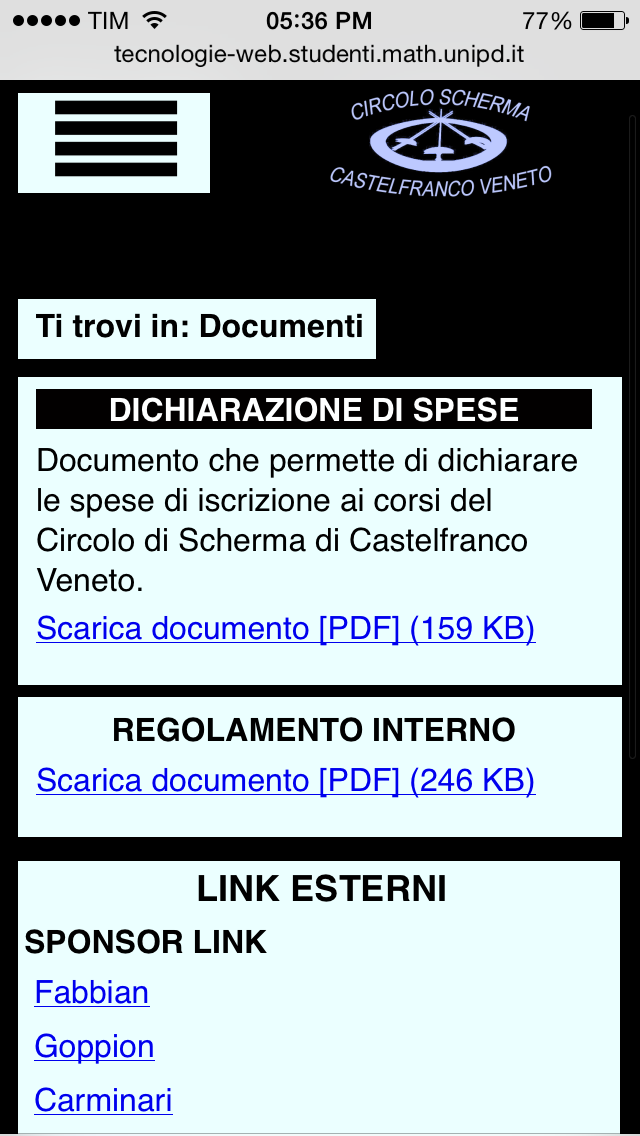
\includegraphics[scale=0.30]{images/articoli_mobile.png}
%		\caption{Screenshot mobile articoli.cgi}
%        \end{subfigure}
%        \caption{Layout schermi diversi}\label{layout}
%\end{figure}



Sono previste inoltre delle variazione del layout nel caso javascript sia disabilitato nel browser client. In particolare nelle pagine di inserimento o modifica della parte amministratore, vengono nascosti i bottoni dei tag speciali e la sidebar con la legenda, per far spazio ad una colonna con le istruzioni per inserire i tag correttamente.

%\begin{figure}[h!]
%        \centering
%        \begin{subfigure}[b]{0.48\textwidth}
%                \includegraphics[width=\textwidth]{images/formJavascript.png}
%                \caption{javaScript abilitato}
%                \label{javascript}
%        \end{subfigure}
%        ~
%        \begin{subfigure}[b]{0.48\textwidth}
%                \includegraphics[width=\textwidth]{images/formNoJavascript.png}
%                \caption{javaScript disabilitato}
%                \label{nojavascript}
%        \end{subfigure}
%        \caption{Layout con/senza javascript}\label{layoutJavascript}
%\end{figure}
\newpage
\section{Accessibilit\`a}
	\subsection{Link nascosti}
Per rendere il sito più accessibile e migliorare la navigazione, in particolar modo per le persone non vedenti o comunque per tutti coloro che utilizzano come supporto uno screen reader, abbiamo deciso di introdurre numerosi link nascosti che consentono di muoversi agilmente all'interno di una determinata pagina web. \\
Ecco nel dettaglio la loro implementazione:
	\begin{itemize}
		\item
		\item
		\item
	\end{itemize}
\subsection{Tab Index}
Un altro meccanismo utilizzato per consentire una migliore esperienza per l'utente è stato quello di personalizzare i tab index in modo che ci si possa muovere più velocemente e senza avere bisogno del mouse.
In particolare gli abbiamo utilizzati per la navigazione nel menù e per i form presenti nella parte amministrativa.

\subsection{Contrasti dei colori}	

\newpage
\section{Validazione}
	\subsection{XHTML e XSL}
	\subsubsection {Falsi positivi}
\subsection{CSS}

\subsection{XML e XSD}
La validazione dei file XML rispetto agli schemi corrispondenti \`e stata effettuata tramite il seguente validatore on-line:
\\
\href{http://www.freeformatter.com/xml-validator-xsd.html}{http://www.freeformatter.com/xml-validator-xsd.html}
\begin{figure}[htbp]
	\centering
	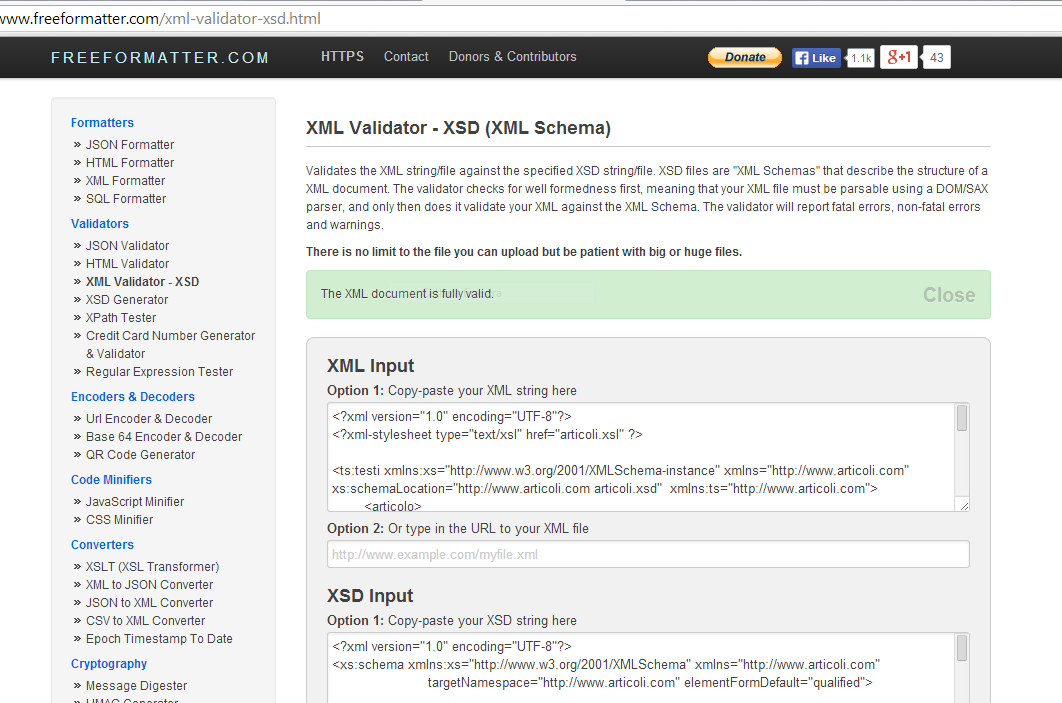
\includegraphics[width=105mm, height=13mm]{images/validazioneArticoli.png}
\end{figure}
Non è stato utilizzato il validatore del W3C poich\`e al momento non era funzionante.
	

\newpage
\section{Compatibilit\`a}
	Riportiamo di seguito, per ogni sistema operativo, i browser dove abbiamo verificato la compatibilit\`a:
\begin{itemize}
		\item WINDOWS
		\begin{itemize}
			\item IEXPLORER 6
			\item IEXPLORER 7
			\item IEXPLORER 8
			\item IEXPLORER 9
			\item CHROME 33
		\end{itemize}
		\item MAC OSx
		\begin{itemize}
			\item
			\item
			\item
		\end{itemize}
		\item LINUX UBUNTU
		\begin{itemize}
			\item
			\item
			\item
			\item
		\end{itemize}
\end{itemize}

\end{document}